%%%%%%%%%%%%%%%%%%%%%%% file typeinst.tex %%%%%%%%%%%%%%%%%%%%%%%%%%%%%%
%
% This is the LaTeX source for the instructions to authors using
% the LaTeX document class SVMultln with class option 'lnicst'
% for contributions to the Lecture Notes of the Institute for
% Computer Sciences, Social-Informatics and
% Telecommunications Engineering series.
% www.springer.com/series/XXXX       Springer Heidelberg 2007/08/05
%
% It may be used as a template for your own input - copy it
% to a new file with a new name and use it as the basis for
% your article. It contains a few tweaked sections to demonstrate
% features of the package, though.
%
% If you have not much experiences with Springer LaTeX support,
% you should better use the special demonstration file "lnicst.tex"
% included in the LaTeX package for LNICST as template.
%
%%%%%%%%%%%%%%%%%%%%%%%%%%%%%%%%%%%%%%%%%%%%%%%%%%%%%%%%%%%%%%%%%%%%%%%%

%\documentclass[lnicst,sechang,a4paper]{svmultln}
\documentclass{llncs} %this is for NSS
\bibliographystyle{splncs}
%\documentclass[runningheads,a4paper]{llncs} 



\usepackage{amssymb}
\setcounter{tocdepth}{3}
\usepackage{graphicx}


%\usepackage{amssymb}
%\setcounter{tocdepth}{3}
%\usepackage{graphicx}
%\usepackage{fancyhdr}
%\usepackage{lastpage}

\usepackage{url}

%\urldef{\mailsa}\path|{alfred.hofmann, ursula.barth, ingrid.haas, frank.holzwarth,|
%\urldef{\mailsb}\path|anna.kramer, leonie.kunz, christine.reiss, nicole.sator,|
%\urldef{\mailsc}\path|erika.siebert-cole, peter.strasser, lncs}@springer.com|    
%\newcommand{\keywords}[1]{\par\addvspace\baselineskip
%\noindent\keywordname\enspace\ignorespaces#1}


%added by the author himself
\usepackage{subfig}
\usepackage[]{algorithmicx}
\usepackage[]{algorithm}
\usepackage{algpseudocode}

\usepackage{color}
%\usepackage[numbers]{natbib}
\usepackage{calc}
\usepackage{siunitx}
\DeclareSIUnit\mt{\milli\tesla} %% A method for say short cut or new unit!
\sisetup{inter-unit-product = {-}}

\newcolumntype{P}[1]{>{\centering\arraybackslash}p{#1}}

\usepackage[T1]{fontenc}
\usepackage[ansinew]{inputenc}
\usepackage[english]{babel}
\usepackage{adjustbox}
\usepackage{amsmath,amsfonts,amssymb}
\usepackage{xparse}
\usepackage[section]{placeins} 
\usepackage[misc]{ifsym}
\usepackage{url}

 
\usepackage[many]{tcolorbox}
\usetikzlibrary{decorations.pathreplacing}

%added by kimmo
%\setlength\parskip{12pt}
%\setlength\parindent{0pt}
%\pagestyle{fancy}
%\fancyhf{} 
%\fancyfoot[C]{\thepage\ / \pageref{LastPage}}
%\renewcommand{\headrulewidth}{0pt}



\begin{document}



\mainmatter  % start of an individual contribution

% first the title is needed
\title{Pseudonym Based Solutions to Defeat IMSI Catchers Can Enable A DoS Attack}
%Concealing IMSI in 5G Network Using Identity Based Cryptography

% a short form should be given in case it is too long for the running head
%\titlerunning{Concealing IMSI Using Identity Based Encryption} 


% the name(s) of the author(s) follow(s) next
%
% NB: Chinese authors should write their first names(s) in front of
% their surnames. This ensures that the names appear correctly inlso
% the running heads and the author index.
%
\author{Mohsin Khan$^\text{1(\Letter)}$%
%%\thanks{Please note that the LNICST Editorial assumes that all authors have used
%%the western naming convention, with given names preceding surnames. This determines
%%the structure of the names in the running heads and the author index.}%
\and Kimmo J\"arvinen$^\text{1}$
\and Philip Ginzboorg$^\text{2,3}$
\and Valtteri Niemi$^\text{1}$
}  %

%\authorrunning{Mohsin Khan \and Valtteri Niemi}

% (feature abused for this document to repeat the title also on left hand pages)

% the affiliations are given next
\institute{$^\text{1}$University of Helsinki, Helsinki, Finland\\
\{\email{mohsin.khan, kimmo.u.jarvinen, valtteri.niemi}\}\email{@helsinki.fi}\\
$^\text{2}$ Huawei Technolgies, Helsinki, Finland\\
$^\text{3}$ Aalto University, Espoo, Finland\\
\email{philip.ginzboorg@huawei.com}
%P.O. Box 68 (Gustaf H\"allstr\"omin katu 2b)\\
%FI-00014 University of Helsinki\\
%Finland\\
%\url{https://www.cs.helsinki.fi/en}
}

%relationship stu
%
% NB: a more complex sample for affiliations and the mapping to the
% corresponding authors can be found in the file "lnicst.dem",
% that is contained in the LNICST LaTeX support package.
%

%%%\toctitle{Lecture Notes in Computer Science}
%%%\tocauthor{Authors' Instructions}
\maketitle


\begin{abstract}
IMSI catchers are still in existence in all the 3GPP defined networks. Pseudonym based solutions to defeat IMSI catchers have been published in the recent years. In these solutions, we have found one vulnerability, that enables an attacker to convince the home network (HN) to forget an old pseudonym of a legitimate UE without any participation of the legitimate UE. A malicious UE or an SN can exploit this vulnerability to kick a legitimate UE out of service. We show that, exploiting this vulnerability, a novel DDoS attack can be mounted against an entire HN. The attack can send 50 percent of the UEs out of service using a reasonably large botnet of mobile users. We justify our claim by an analytical argument backed by a simulation. We present a solution to fight against the DDoS attack by using the location update message sent by an SN to an HN. We argue that our solution is immune to the the DDoS attack, protects the identity privacy, and remains backward compatible. In principle, a malicious SN can still mount a DoS attack against our solution. However, we argue that the SN can not gain anything meaningful before the DoS attack is detected and stopped. Besides, an SN can behave maliciously in other, even more fatal ways. We also discuss other practical issues of the usability of pseudonyms from charging and lawful interception point of view that appear to be ignored so far.
\keywords{3GPP $\cdot$ IMSI catchers $\cdot$ Pseudonym $\cdot$ Identity $\cdot$ Privacy}
\end{abstract}


\section{Introduction} \label{intro}
International mobile subscriber identity (IMSI) cathers are threats to the identity privacy of mobile users. Passive IMSI catchers are devices that observe the wireless traffic and store all the IMSIs observed. Active IMSI catchers are malicious devices that can trick a user equipment (UE) to reveal its IMSI. Protection against passive IMSI catchers have been in the cellular networks since the second generation (GSM). However, active IMSI catchers have persisted in all the cellular networks, namely, GSM, UMTS and LTE \cite{mobicom95,imsi_catcher_report_bochum,Ginzboorg_Niemi_2016,washingtonpost2014,pets2017,pki_umts_imsi_catcher}. 

\subsubsection{IMSI Catching}
The network a UE has a subscription with is called the home network (HN). The network a UE visits and gets service from is called serving network (SN). In an ideal situation, a UE has to identify and authenticate itself to an SN before receiving any services from it. In cellular networks the encryption key in a UE is generated using the pre-shared symmetric key during authentication \cite{TS33401}. So, before authentication, neither a UE nor the SN/HN knows the key to use for encryption or decryption.  Consequently, the identity of the UE has to be sent in plaintext to the SN. This enables an active IMSI catcher to play its trick.

The trick an IMSI catcher play against the UEs is that, it impersonates a legitimate SN and ask for the identity of all the UEs in the range of the IMSI catcher. The UEs has no way to differentiate an IMSI catcher from a legitimate SN, hence reveal their IMSIs as if they were revealing to a legitimate SN. 

An IMSI catcher can exploit the knowledge of caught IMSIs to monitor and track the physical location of a mobile user \cite{tracking_bins,goldman2007mobile}. Please note that the term "IMSI catcher" is also used in a wider meaning, referring to extended attacks, including man-in-the-middle type of attacks or just spamming \cite{catch_me_if_you_can,chinese_spam}. In this paper we limit our discussion only to prevent the IMSI catchers from catching the IMSIs (identities) of the users.

Different kind of solutions to defeat IMSI catchers have been proposed over the years \textcolor{red}{cite}. In addition to protect privacy, a desirable property of the solution is backward compatibility, i.e., it should protect the identity privacy even in the presence of a legacy SN. This is because, if the solution to defeat IMSI catchers works only in the latest generation of cellular network (e.g., 5G), then an attacker can mount a downgrade attack. 

\subsubsection{Pseudonym Based Solutions}
A potentially simple and backward compatible approach is to use frequently-changing temporary identities for mobile users \cite{CCS15,SSR15,Ginzboorg_Niemi_2016,Norrman_Naslund_Dubrova_2016,yemen2017}. The idea is, even if an IMSI catcher play its trick, only the temporary identity of a UE would be revealed. So, the IMSI catcher would not be able to associate the temporary identity with any user who is previously known or will be known in the future. The temporary identities are called pseudonyms, hence the solutions use this approach are called pseudonym based solutions. 

In 2015, Borek, Verdult, and Ruiter \cite{CCS15} and Khan and Mitchell \cite{SSR15}, described pseudonym based solutions that have the same format as IMSIs. From now on we will refer these two schemes as BVR and KM15 schemes. These solutions are sensitive to the loss of synchronization between the pseudonyms in the UE and the HN. In the worst loss of synchronization case, there is not even one pseudonym left in the UE that the HN accepts. Hence all the identification and authentication attempt would fail thereafter and the UE would go out of the service. There is a vulnerability in these solutions that can be exploited by an attacker to cause the loss of pseudonym synchronization. The attacker can be a malicious UE or a malicious serving network (SN).

In 2017, Khan and Mitchel \cite{wisec17} identified the loss of synchronization problem caused by a UE and proposed a solution. In the rest of the paper we will refer to this solution as KM17 scheme. Careful investigation into this scheme shows that a UE has to use one pseudonym at least twice before it can get a new pseudonym from the network. The authors also argue that their solution is not immune to a malicious SN. To address the issue of malicious SNs, they introduce an identity recovery procedure. But this procedure adds complexity: the number of temporary identities per user increases from two to six. Moreover, as we explain, the recovery mechanism itself can be exploited by an IMSI catcher to track the mobile user.

%\begin{figure}[!tbp]
%  \centering
%  \begin{minipage}[b]{0.44\textwidth}
%    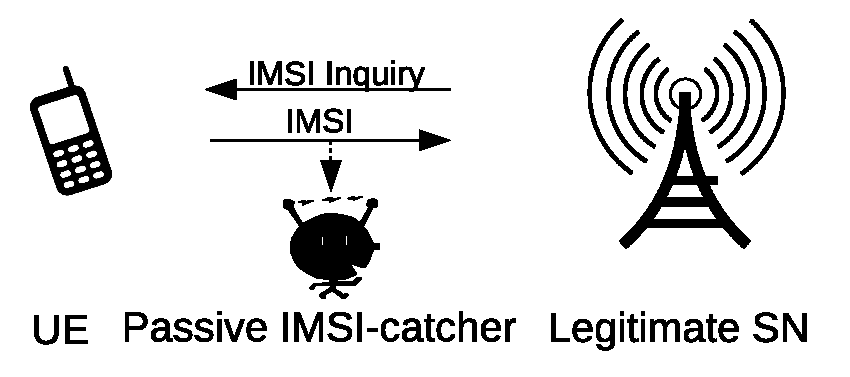
\includegraphics[width=\textwidth]{Passive_IMSI-Catcher.eps}
%    \caption{Legitimate SN}
%  \end{minipage}
%  \hfill
%  \begin{minipage}[b]{0.50\textwidth}
%    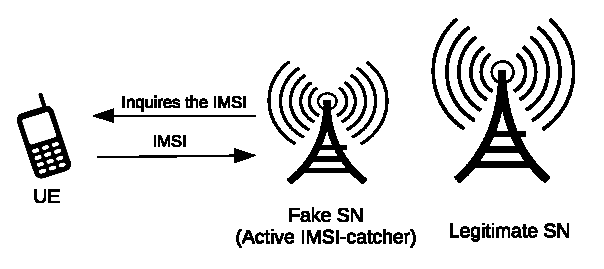
\includegraphics[width=\textwidth]{Active-IMSI-Cactcher.eps}
%    \caption{IMSI-catcher}
%  \end{minipage}
%  \caption{IMSI-catcher}
%  \label{fig:IMSI-catching}
%\end{figure}

\subsubsection{Our Contribution}
We propose a pseudonym based solution that builds on top of those in BVR, KM15 and KM17 schemes. The following contributions are made:
\begin{enumerate}
\item We have identified weaknesses in KM17 scheme
\item We show that a DoS attack can be mounted against an entire HN using the vulnerability identified in \cite{wisec17}. We calculate the expected success rate of the attack and argue that the attack can be fatal in practice.
\item We show how the pseudonyms synchronization can be handled in a simple manner (also when there are DoS attacks), with three pseudonyms per user instead of six. In our solution, a UE can get a new pseudonym after using an old pseudonym only once in a successful AKA instead of twice.
\item Using probabilistic analysis, we show that a malicious SN can not mount any meaningful attack against our solution as long as synchronization of pseudonyms is the concern.
\item We discuss some practical concerns of using pseudonyms instead of IMSIs from billing and lawful interception point of view and suggest solutions.
\end{enumerate}




\section{Preliminaries}

\begin{enumerate}
 \item AUTS
 \item IMSI space, MSIN space
 \item let $\mathcal{M}$ be the MSIN space. $\mathcal{M}$ can be $10^10$ or $10^9$
 \item $n$ is the number of subscribers
\end{enumerate}


\subsubsection{Identification in the existing networks}
\subsubsection{Authentication in the existing networks} we need to discuss the authentication mechanism because the pseudonym based approach uses the messages in the authentication protocol to piggyback the messages required to be sent across.

\section{Related Work}
The idea of using pseudonyms to secure identity privacy has been used since the GSM network \textcolor{red}{cite}. However, the practice of using pseudonyms has been limited only by a UE and the SN. When a UE visits an SN, after the idenfication, if the authentication (UMTS AKA, LTE AKA) runs successfully, the SN assigns the UE a pseudonym with confidentiality protection. This pseudonym (known as TMSI in GSM and UMTS, and as GUTI in LTE) \textcolor{red}{cite} is used thereafter by the UE whenever an identification is required. The use of TMSI and GUTI has been successful in the protection against passive IMSI catchers \textcolor{red}{cite}.

However, an SN can still make an IMSI inquiry to a UE because of losing the TMSI/GUTI or just because the UE is visiting the SN for the first time.  Since an active IMSI catcher can impersonate a legitimate SN, an IMSI catcher too, can make an IMSI inquiry. The UE does not know if the inquiry is coming from an attacker or a legitimate SN. Hence, the UE responds to the inquiry with the IMSI. The BVR and KM schemes describes how the use of HN recongnized pseudonym can be introduced in the legacy networks. Following the BVR and KM schemes in 2015, there have been few other proposals \cite{Ginzboorg_Niemi_2016,Norrman_Naslund_Dubrova_2016,yemen2017} published in 2016 and 2017. All these proposals use essentially the same idea of using frequently changing pseudonyms recongnized by the HN. The vulnerability identified in \cite{wisec17} is present in all these solutions. So, for simplicity and limitation of space, we explain only one of these schemes briefly and present our attack and solution in the context of the chosen scheme. We choose the BVR scheme.

\subsection{BVR Scheme}
They pseudonym used in this scheme is called pseudo mobile subscriber identifier (PMSI). Besides the shared secret $\mathcal{K}$, every user shares another secret key $\kappa$ with the HN. The SIM inside the UE stores two pseudonyms at any point of time, $\left(PMSI,P_{new}\right)$. The SIM uses $P_{new}$ the next time the UE receives an IMSI inquiry and keep using $P_{new}$ untill it receives a new pseudonym. The HN also stores two pseudonyms $\left(p,p'\right)$ for every subscriber at ay point of time. In an ideal situation, $PMSI = p$ and $P_{new} = p'$. 

The HN sends the next pseudonym encrypted by the key $\kappa$ as a part of the random challenge $RAND$ used in AKA. Upon the successful and positive completion of the AKA between the SN and the UE, the next pseudonym can be decrypted by the SIM. The BVR scheme builds on top of the UMTS AKA. Figure \ref{fig:bvr_solution} shows the requried changes. Comparaing Figure \ref{fig:umts_AKA} and \ref{fig:bvr_solution} shows that no changes are made in the messages that are transmitted, but only in the end points, i.e., the SIM and the HN. Since both of the HN and the SIM are maintained by same entity, the scheme is transparent to the legacy SNs.


\begin{figure}[]
  \centering
    \includegraphics[width=\textwidth]{BVR.eps}
  \caption{The BVR Scheme}
  \label{fig:bvr_solution}	
\end{figure}


\subsubsection{Vulnerability in BVR Scheme}
Note that, whenever an AV request arrives for $p'$, the HN forgets $p$. Forgetting an old pseudonym is important so that it can be reused. But forgetting before being confirmed that $p'$ has been received by the UE is a vulnerability as pointed in the \cite{wisec17}. If a fake UE (FUE) identifies itself using a random pseudonym and if by chance, the random pseudonym is associated with a legitimate UE, the HN forgets an old pseudonym for the legitimate UE. The network also computes a new pseudonym which the legitimate UE has no knowledge of. If the network remembers  $k$ number of pseudonyms before forgetting any, the FUE needs to make the attack $k$ times so that the network forgets all the pseudonyms that the legitimate user possesses. So, in the case of BVR scheme, the FUE has to send two pseudonyms. This is a fatal damage to the identity of the UE, because all the successive authentications of the UE will fail. In Section \ref{sec:attack} we will show how this vulnerability can be exploited into a fatal DoS attack.


\subsection{KM17 Scheme}
In KM17, the authors have used the location update message sent by an SN to an HN after successful and positive completion of AKA as the confirmation that the UE has received $p'$. The scheme uses three pseudonyms in the HN instead of two. It also uses three recovery identities (RID), that we will discuss in the following section.


\subsubsection{Weaknesses in KM17 Scheme}
Careful investigation in KM17 scheme shows that a pseudonym has to be used at least two times before the UE can get a new pseudonym from the HN. The scheme maintains three pseudonyms $p_{past},p_{current}$ and $p_{future}$ at the HN end. The HN always embeds encrypted $p_{future}$ (generates a new one if $p_{future}$ is null) in the RAND. The HN forgets $p_{past}$ only when a location update for $p_{future}$ arrives at HN. A location update for $p_{future}$ would arrive only if $p_{future}$ was used by the UE already at least once. After receiving the location update for $p_{future}$, the HN updates $p_{past} \leftarrow p_{current}$, $p_{current} \leftarrow p_{future}$ and $p_{future} \leftarrow null$. Now, the UE has to use $p_{current}$ to get a new pseudonym from the HN. Notice that the $p_{current}$ after the location update is same as the $p_{future}$ before the location update arrived. Consequently, our claim follows.

The authors argue that the scheme is not immune to malicious SN who tries to attack by sending fake location update message. As a reactive measure, the authors propose a recovery process that enables a UE and the HN to get back in a synchronized state of pseudonyms. The scheme uses temporary recovery identity (RID). The HN sends the RID as a part of the RAND in a similar way a pseudonym is sent. When a UE gets convinced that the pseudonym synchronization has been lost, the UE sends the RID piggybacked in the reject message AUTS. Based on the RID, the process can recover to a synchronized pseudonym state. Detail of the process can be found in \cite{wisec17}. However, an IMSI catcher can convince a UE that the synchronization has been lost and learn the RID of the UE. Now the IMSI catcher can track the user using this RID instead of IMSI. This argument shows that the pseudonyms used in this scheme are as good as frequent the RIDs are changed. 

However, one might argue that the RIDs can be changed as frequent as the pseudonyms are changed. Note that, forgetting an old RID is also triggered by the same location update message that triggers forgetting an old pseudonym. Consequently, synchronization of RIDs become as vulnerable as synchronization of pseudonyms, when a malicious SN sends fake location update message.

\section{Attack On BVR Scheme} \label{sec:attack}
The attack is mounted by an FUE. The attack has two phases.

\subsubsection{Phase 1} \label{sec:attac_fue_phase1}  FUE sends an attach request using a random pseudonym $q_1$ to a legitimate SN. The legitimate SN sends a AV request for $q_1$ to the HN. If by chance, $q_1 = s_{p'}$, the HN forgets $s_p$ and sets $s_p \leftarrow s_{p'}$. The HN also generates an unused pseudonym ${p''}$ and sets $s_{p'} \leftarrow p^{''}$. As a result, in the HN, the current  pseudonym-state for the subscriber $s$ is $\left(s_{p} = P_{new},s_{p'} \neq PMSI,P_{new}\right)$. Now, there is only one pseudonym present both at the UE and HN. See Figure \ref{fig:dos_attack}.

\subsubsection{Phase 2} \label{sec:attac_fue_phase2} The FUE sends another attach request using a random pseudonym $q_2$ to a legitimate SN. The legitimate SN sends a AV request for $q_2$ to the HN. If again by chance, $q_2 = s_{p'}$, then the HN again forgets $s_{p}$, sets $s_p \leftarrow s_p'$. HN also generates an unused pseudonym $p'''$ and sets $s_{p'} \leftarrow p'''$. Consequently, the current pseudonym-state of subscriber $s$ is $\left(s_{p} \neq PMSI,P_{new},s_{p'} \neq PMSI,P_{new}\right)$ in the HN. See Figure \ref{fig:dos_attack}

\begin{figure}[]
  \centering
    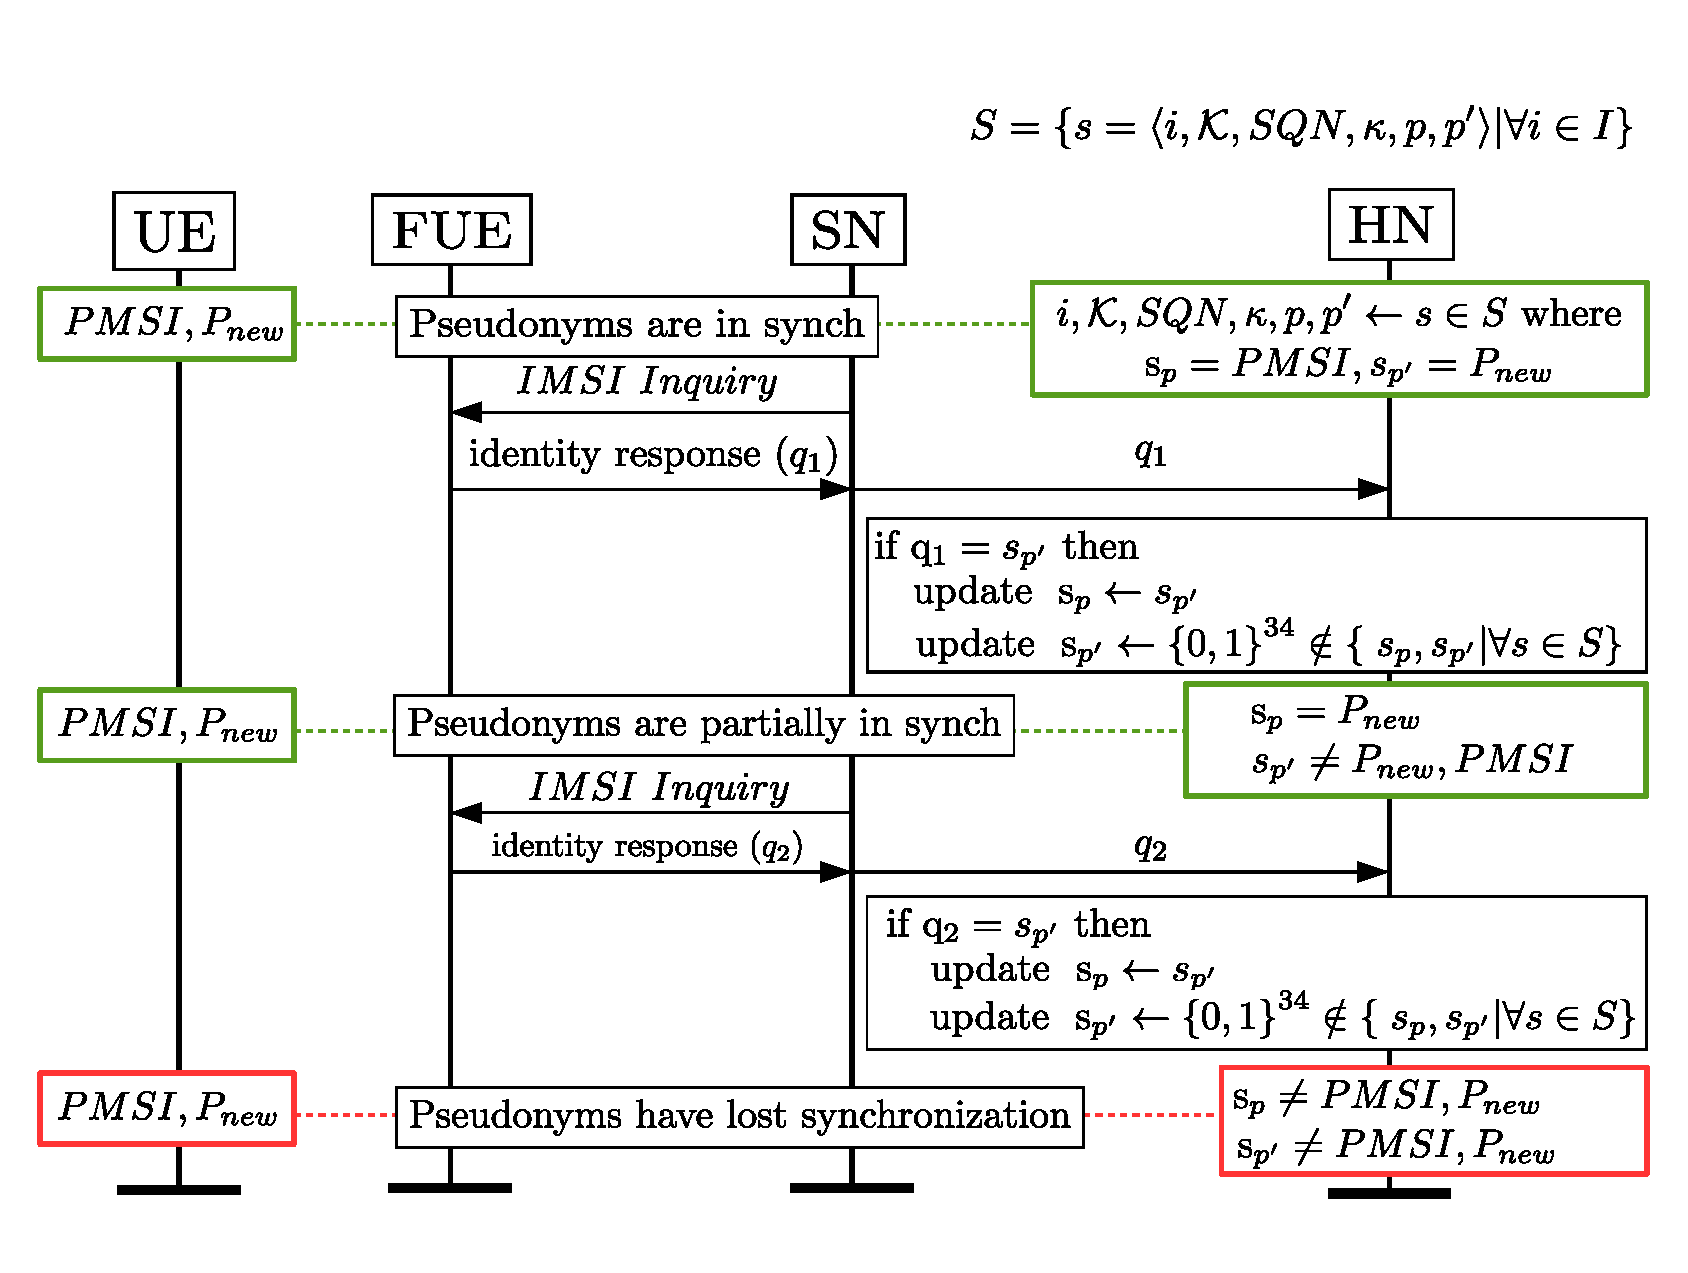
\includegraphics[width=.9\textwidth]{DDoS.eps}
  \caption{A DoS Attack against the BVR scheme}
  \label{fig:dos_attack}	
\end{figure}

The next time the user would need to authenticate itself to a network, the authentication will fail and hence be denied any service. In this attack, it is assumed that the UE has not obtained a new pseudonym via a legitimate SN while the attack was mounted.

\subsection{The DDoS Attack Against the BVR Scheme} \label{sec:ddos_attack}
If the probability of success of the above attack to a targeted user is $\frac{1}{10^{20}}$. The probability of success of the attack to any user is $\frac{n}{10^{20}}$. This is a tiny probability, but by attacking many times, we can obtain a significant number of affected users. This can be achieved by deplyoing a botnet of mobile phones into a DDoS attack on the HN.

In the DDoS attack, the mobile bots send many attach requests using different pseudonyms to legitimate SNs. The legitimate SNs in turn sends AV request for those pseudonyms to the HN. Let us assume, the total number of pseudonyms sent to the HN is a large integer $m$. In this case, a user $s$ will be affected by the attack if there exists two integers $0 < x < y \leq m$ such that $q_{x} = s_{p'}$ and $q_{y} = s_{p'}$. 

We have considered two different ways to mount this attack. In one way, the pseudonyms used in the attach requests are chosen randomly with replacement, which means the attack might sent one pseudonym more than once to the HN. In the other way, the pseudonyms are chosen without replacement, which means the attack send one pseudonym only once.

\subsubsection{With Replacement}
In this case, after sending $m$ number of pseudonyms to the HN, the expected portion of affected users $E[u_a]$ is
\begin{eqnarray}
E\big[ u_a \big] &=& \left(1- \left(1 - \frac{1}{\mathcal{M}}\right)^m - m\left(\frac{1}{\mathcal{M}}\right)\left(1 - \frac{1}{\mathcal{M}}\right)^{\left(m-1 \right)} \right) \label{eqn:avg_with_replacement}
\end{eqnarray} 

See Appendix \ref{appendix: A} for the derivation. We have run a simulation of this attack and found that above model is fairly accurate. See Figure \ref{fig:simulation_and_modeling}.


\begin{figure}[]
  \centering
  \begin{minipage}[b]{0.49\textwidth}
    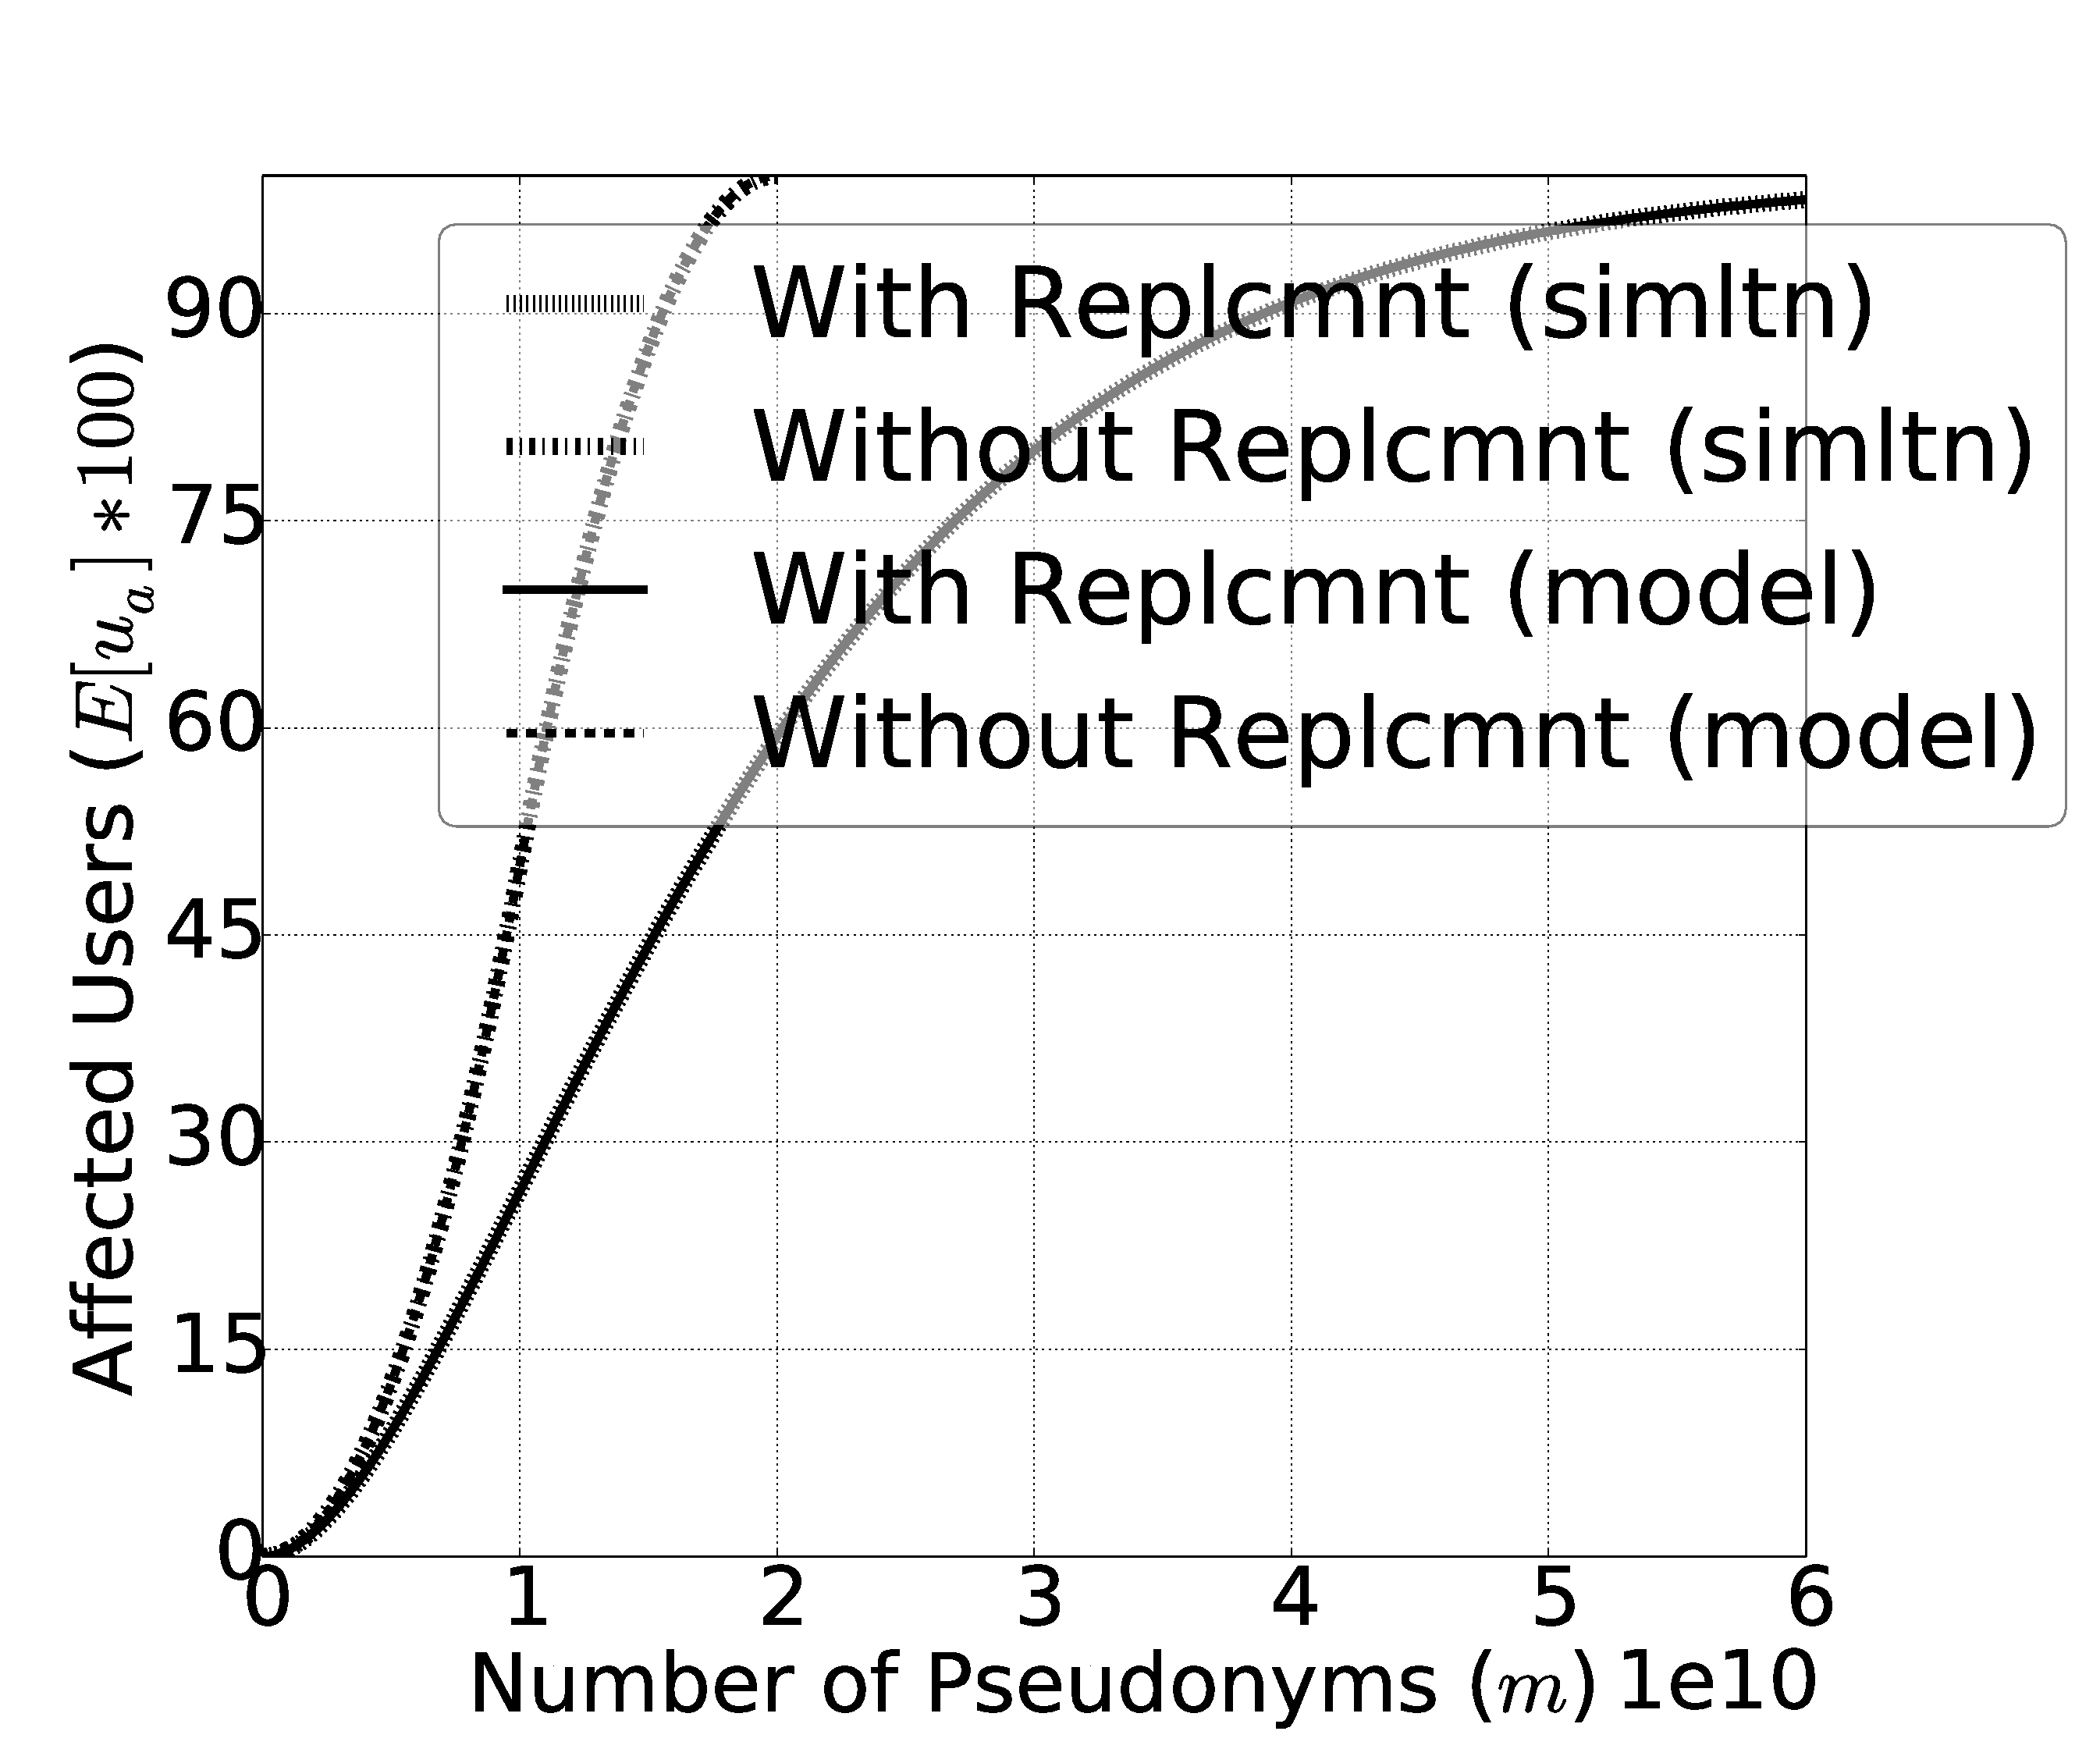
\includegraphics[width=\textwidth]{sim_and_mod.pdf}
   \caption{DDoS Attack. $ \mathcal{M} = 10^{10}, n = 10^{7}$. The model fits so well that it is difficult to distinguish the empirical lines from the model.}
\label{fig:simulation_and_modeling}
  \end{minipage}
  \hfill
  \begin{minipage}[b]{0.49\textwidth}
    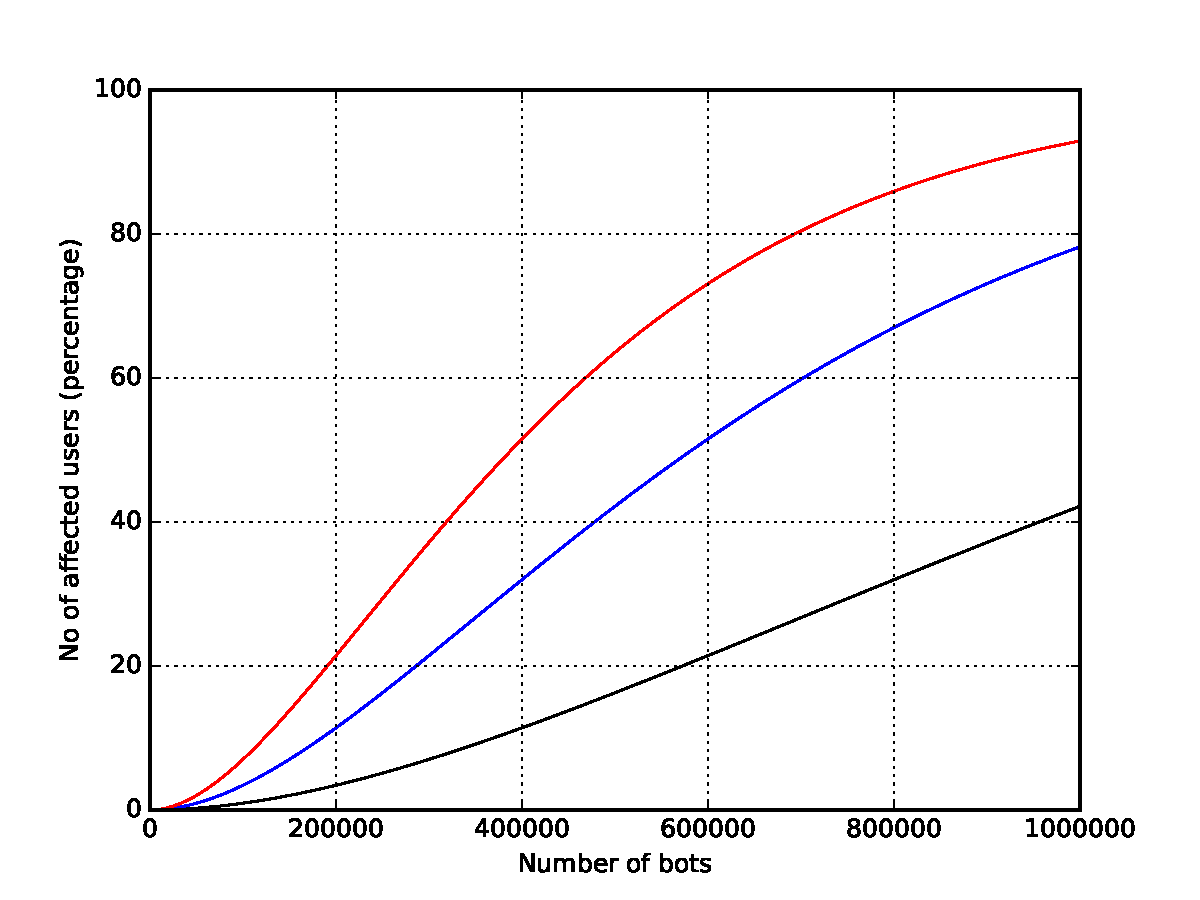
\includegraphics[width=\textwidth]{botplot.pdf}
    \caption{DDoS Attack (with replacement), $\texttt{botnet}_{\texttt{size}} = 10^6$. Different lines represent the success rate as $\texttt{bot}_{\texttt{load}}$ varies.}
  \label{fig:botplot}
  \end{minipage}
\end{figure}

\subsubsection{Without Replacement}
In this case the attacker runs two rounds of the attack. In the first round the attacker sends all the pseudonyms in the IMSI space without replacement, means each pseudonym is sent exactly once. Once the first round is completed, the attacker runs the attack for one more round. However, after sending $m$ number of pseudonyms to the HN, the expected portion of affected users $E[u_a]$ is
\begin{eqnarray}
E\big[ u_a \big] = \begin{cases} \frac{1}{\mathcal{M}}\frac{m^2}{2\cdot \mathcal{M}} & \mbox{if } 0 < m \leq \mathcal{M} \\ 
\frac{1}{\mathcal{M}}(2m - \mathcal{M} - \frac{m^2}{2\mathcal{M}}) & \mbox{if } \mathcal{M} < m \leq 2\mathcal{M} \end{cases}
\label{eqn:without_replacement}
\end{eqnarray} 

See Appendix \ref{appendix: A} for the derivation. We have run a simulation of this attack and found that above model is fairly accurate. See Figure \ref{fig:simulation_and_modeling}. Note that, this is an estimation where the without-replacement attack is not a distributed attack. Rather the attack is mounted by only a single FUE. In the case of distributed and without replacement attack, the expected perecentage of affected users will be less than what is shown in the plot. However, we believe that, the distributed and without replacement attack will have higher number of affected users than that of distributed with-replacement attack. However, it can be a strategic decision of the attacker to choose the value of $\texttt{bot}_{\texttt{load}}$.


\subsection{How Fatal The DDoS Attack Can be In Practice} \label{sec:how_fatal_ddos}
The intensity of the attack in practice will heavily depend on two parameters. The first one is the size of the botnet, we name as $\texttt{botnet}_{\texttt{size}}$. The second one is the number of pseudonyms a bot sends per unit time in the attach requests, we name as $\texttt{bot}_{\texttt{load}}$. According to a thesis conducted in Lund University in 2016 \cite{thesislund}, the EPS AKA has the latency of $550$ milliseconds even when the MME is far away (10,000 km) from the HN. So, the peak value of $\texttt{bot}_{\texttt{load}}$ can safely be considered as $1$ pseudonyms/second, i.e., 3600 pseudonyms/hour.

Mobile botnets are on the rise \cite{botnet_ccs09_symbian,botnet_usenix11,botnet_australia_2016}. Many mobile botnets have already been observed, e.g., Geinimi \cite{botnet_geinimi10}, Zeus \cite{botnet_zeus11}, AnserverBot \cite{botnet_anserverbot}, DreamDroid \cite{botnet_dreamdroid11}. A detailed survey of the state of mobile botnets can be found in \cite{botnet_threat15}. In 2011, it was estimated that Dreamdroid was installed on 120,000 mobile devices \cite{botnet_dreamdroid11}. In 2014, a mobile botnet of 650,000 mobile phones made an attack to a server \cite{chinese_spam}. It would not be surprising if we see a mobile botnet consisting tens of millions of mobile bots in near futrue. However, for the discussion of this paper, we conservatively set the variable $\texttt{botnet}_{\texttt{size}} = 1$ million ($10^6$). See Figure \ref{fig:botplot}, it shows how efficient a botnet of size $10^6$ can be for varied values of $\texttt{bot}_{\texttt{load}}$.



\begin{figure}[]
  \centering
    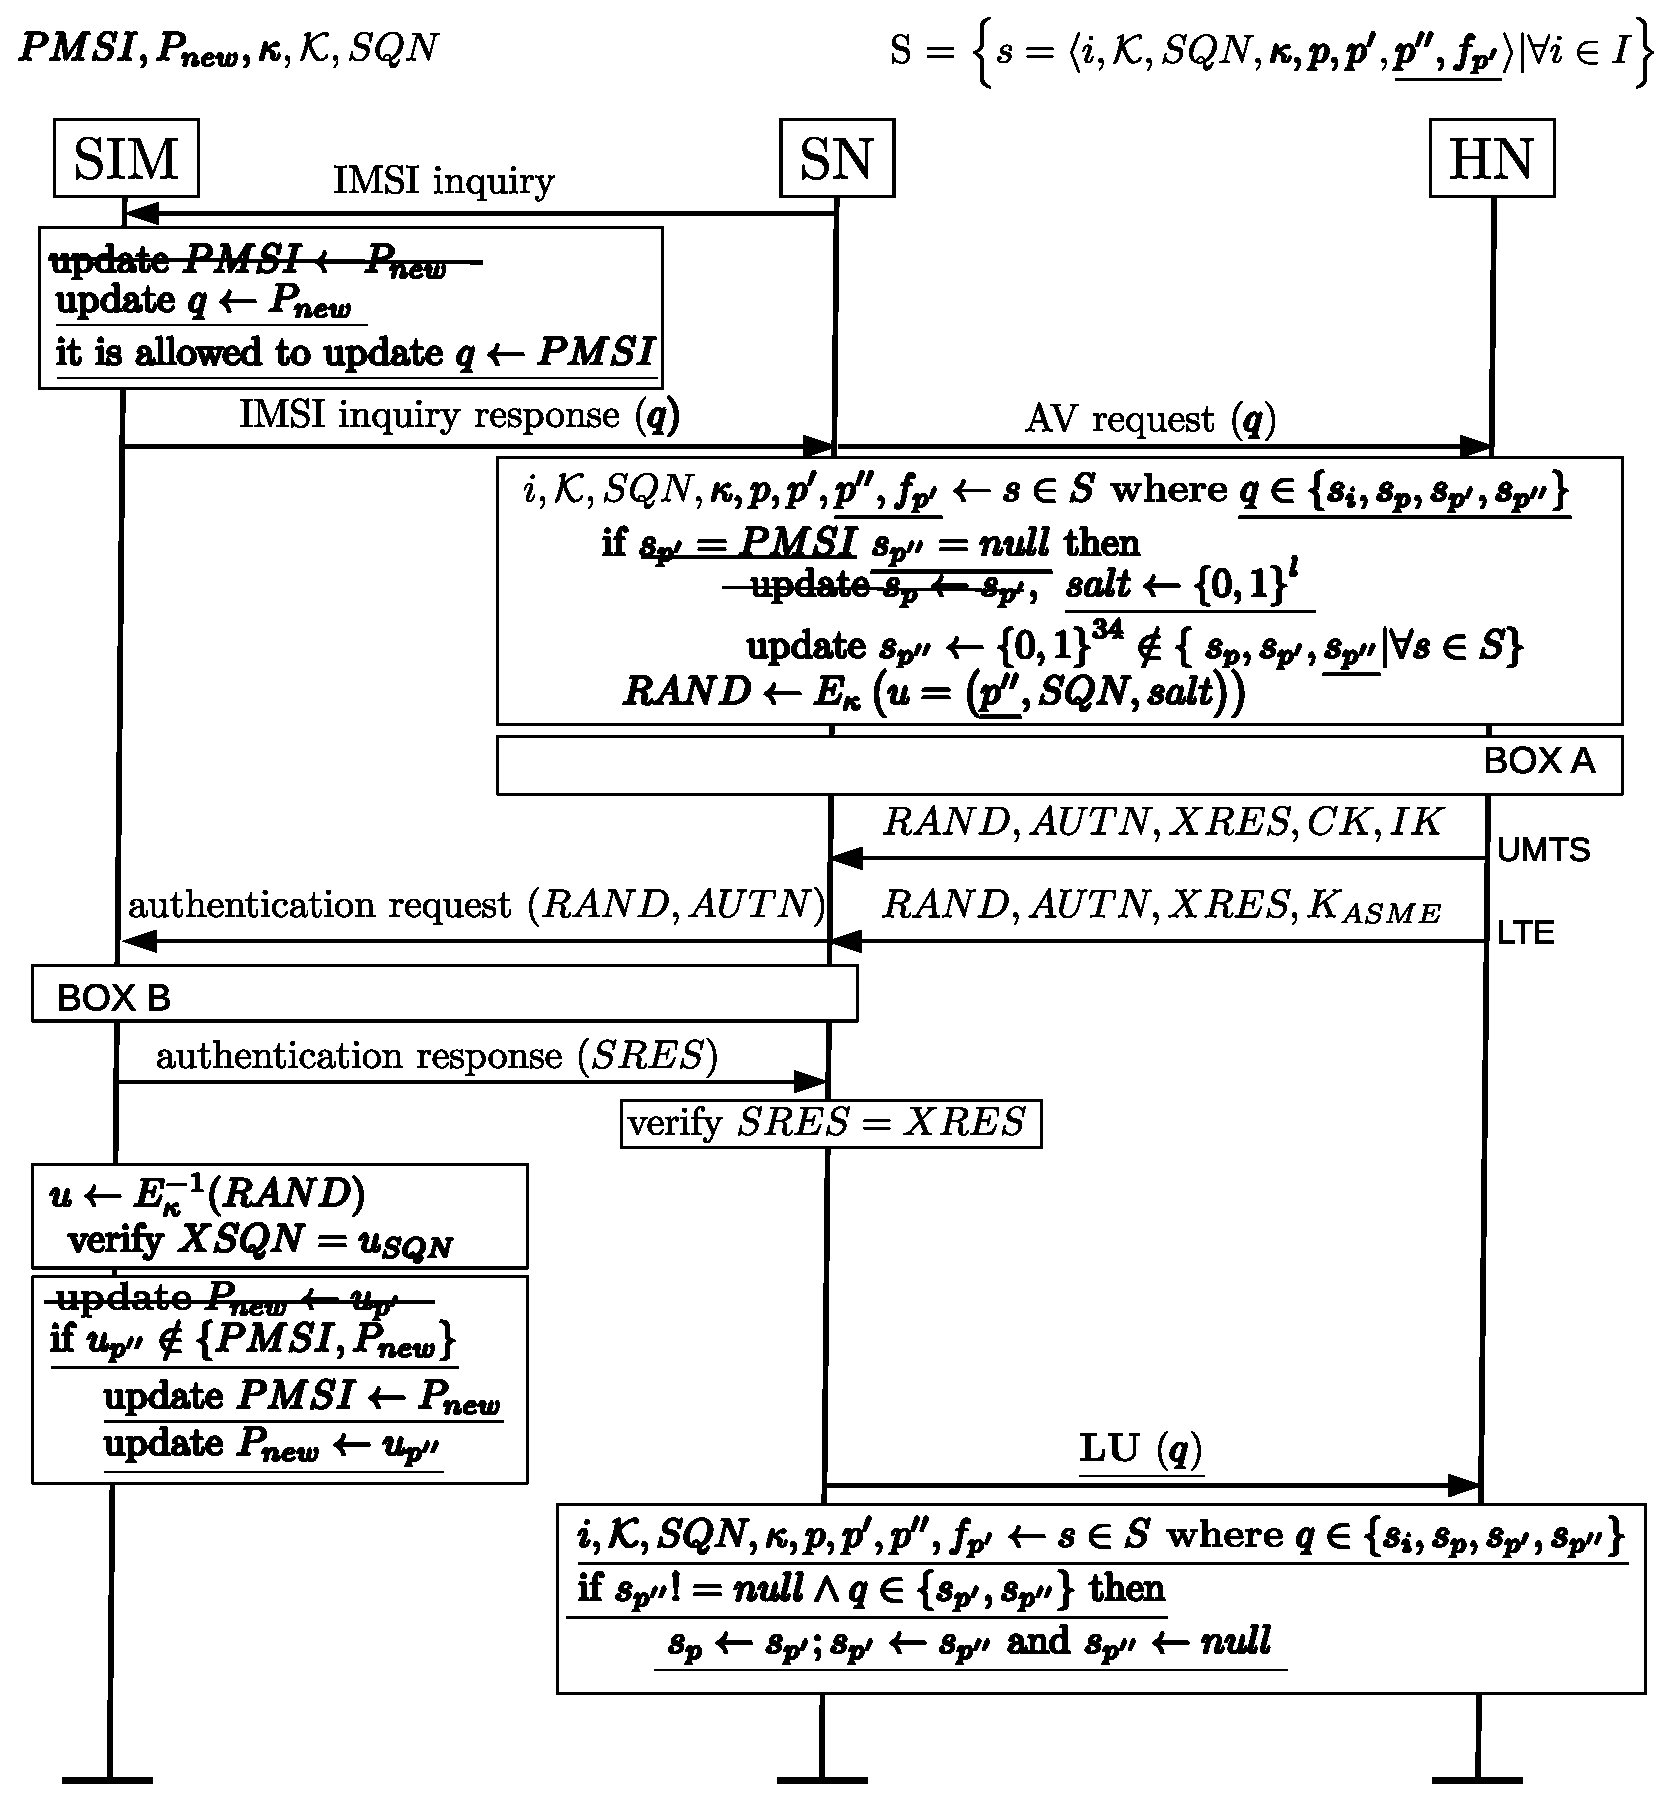
\includegraphics[width=\textwidth]{solution.eps}
  \caption{Solution}
  \label{fig:solution}	
\end{figure}

\section{Our Solution}
As in \cite{wisec17}, our solution also uses the location update message sent by an SN to the HN after the successful and positive completion of an AKA. In the legacy networks, the location update message is sent for an IMSI. As the pseudonyms and IMSIs are not distinguishable by an SN, the location update messages will be sent by an SN for the pseudonyms too. Let us assume that for a subscriber $s \in S$ an AV request has arrived using the pseudonym $p$ and the HN has responded with an AV by embedding $p'$ in the RAND. When a location updated for pseudonym $p$ arrives, the HN considers it as the guarantee that pseudonym $p'$ has arrived in the UE of user $s$.

In the HN, for a user $s \in S$, our solution stores the IMSI $i$ and three pseudonyms $p,p',p''$. In the UE of the user $s$, two pseudonyms $PSMI,P_{new}$ are stored. In an ideal situation $PMSI = p, P_{new} = p'$. We build our solution on top of the BVR scheme. Figure \ref{fig:solution} presents our solution. The bold texts present the changes over UMTS. The bold stricken out texts present the parts that we have discarded from the BVR scheme. The bold and underlined texts present the parts that we have added. 


\subsubsection{At HN side}
Whenever an AV request is received for a subscriber $s$, using any of its identity, i.e., $i,p,p'$ or $p''$, the HN responds with an AV that contains a pseudonym $p''$ in the RAND. If $p''$ is $null$ then an unused pseudonym is chosen and set as $p''$. When $p''$ is not null and a location update message arrives using any of the identities $p',p''$, the HN forgets $p$ by setting $p \leftarrow p', p' \leftarrow p''$ and $p'' \leftarrow null$. 


\subsubsection{At UE side}
If $MAC$ and $SEQN$ verification is successful then the UE verifies if $u_{SEQN}$ is the same as the $XSEQN$. If this verifications is also successful, then the UE sends the SRES to the SN, and sets $PMSI \leftarrow P_{new}$ and $P_{new} \leftarrow u_{p''}$


\section{Analysis of Our Solution}
In order to analyze our solution, we categorize all the possible states of HN in four categories. Based on these four categories, we draw a state diagram as presented in Figure \ref{fig:hn_diagram}. 

\begin{figure}[!tbp]
  \centering
    \begin{minipage}[b]{\textwidth}
    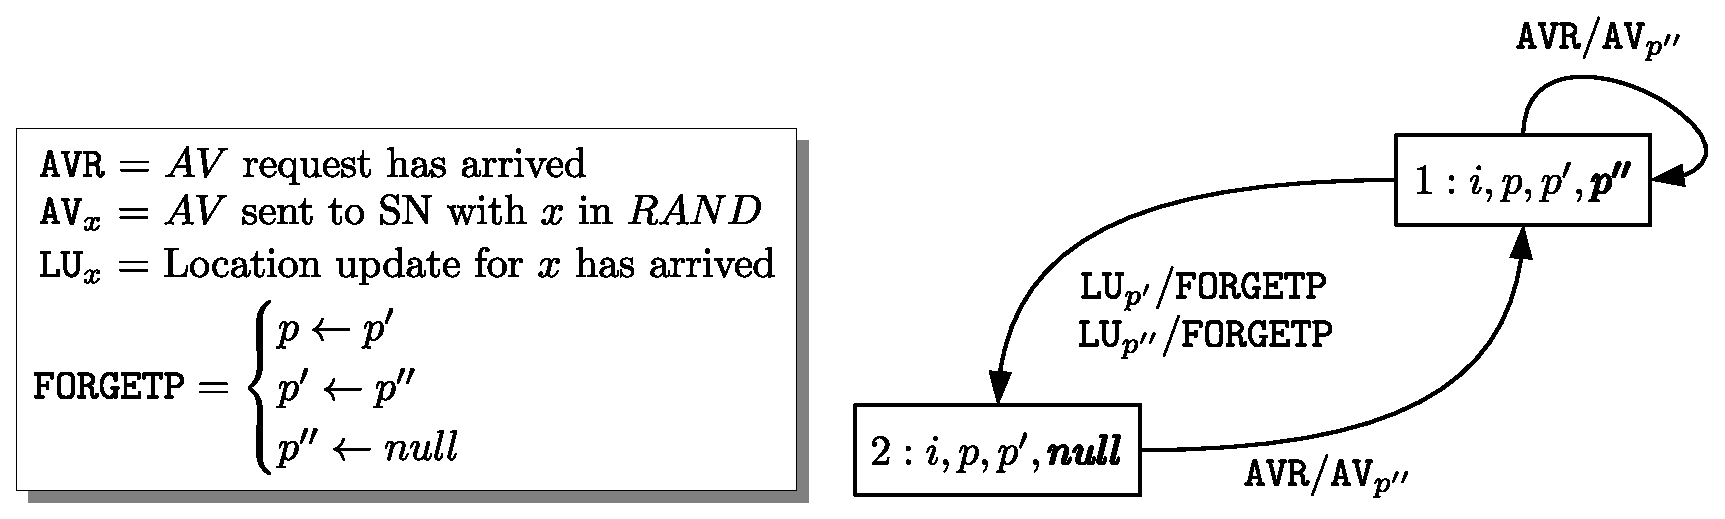
\includegraphics[width=\textwidth]{HN_diagram.eps}
 \caption{State diagram of the solution for a user $s \in S$ at the HN end.}
  \label{fig:hn_diagram}
  \end{minipage}
    \hfill
  \vspace{.5cm}
  \begin{minipage}[b]{\textwidth}
    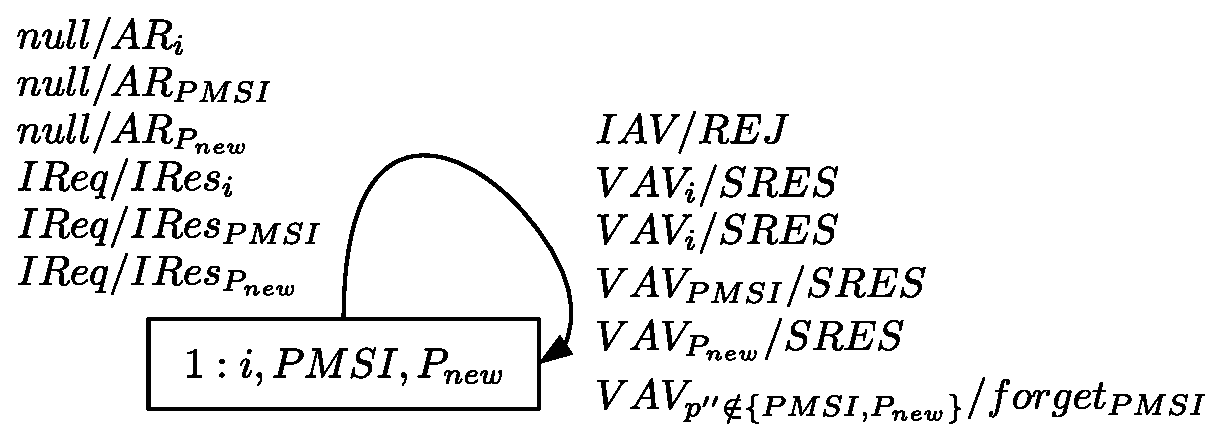
\includegraphics[width=\textwidth]{UE_diagram.eps}
 \caption{Possible cases at at the UE of a user $s \in S$ end. Note that the UE has no knowledge about the cases. All a UE knows are two pseudonyms $PMSI,P_{new}$}
  \label{fig:ue_diagram}
  \end{minipage}
\end{figure}



\begin{figure}[!tbp]
  \centering
    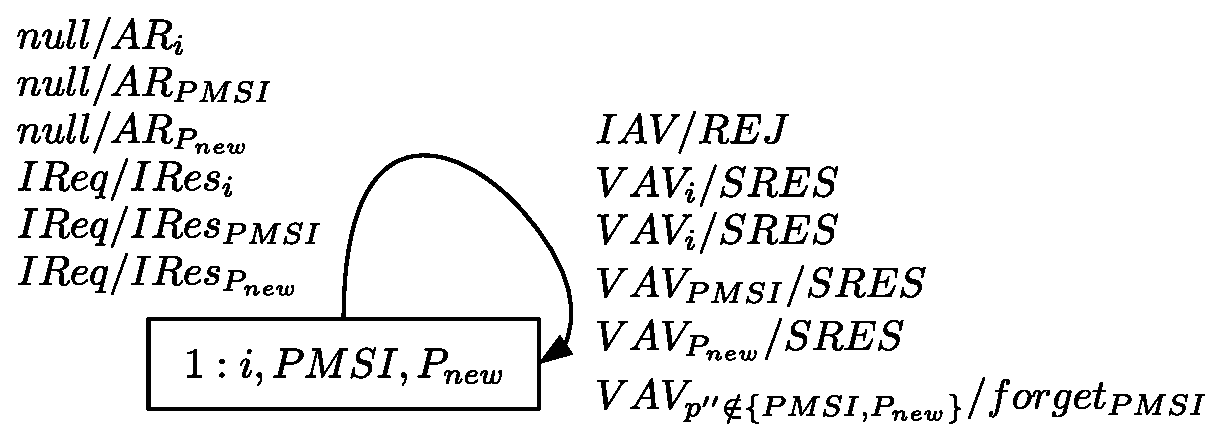
\includegraphics[width=\textwidth]{UE_diagram.eps}
 \caption{Possible cases at at the UE of a user $s \in S$ end. Note that the UE has no knowledge about the cases. All a UE knows are two pseudonyms $PMSI,P_{new}$}
  \label{fig:ue_diagram}
\end{figure}

\begin{enumerate}
 \item discuss the replay attack by the UE
 \item what if AKA is successful but pseudonym is in wrong format?
 \item discuss the case where the SN gets multiple AVs
 \item Comparing the changes with the BVR scheme and the UMTS AKA, one can see that changes are made only in HN and UE. Moreover, no changes are made in the existing message format, hence the solution is still
\end{enumerate}





\subsection{Propoerties of Our Solution}
\subsection{Protects Identity Privacy}
\subsection{Protects against a mobile botnet}
\subsection{Protects against a malicious SN}

\subsection{Solution}
In our solution, each subscriber $s$ keeps record of the IMSI $i$ and two pseudonyms $PMSI,P_{new}$. The HN keeps record of the IMSI $i$, three pseudonyms $s_p,s_{p'}$ and $s_{p''}$. We also introduce one binary flag $LUF_{p'}$ associated with every subscriber $s$ at the HN end. Along with the location udpate message, an SN also sends the pseudonym of the involved subscriber.  $LUF_{p'}$ is set to $1$ if the HN has already received a location update message for the pseudonym $s_{p'}$. The flags are set to $0$ otherwise. In the begining of the life of a SIM card, it stores the IMSI and two pseudonyms $PMSI$ and $P_{new}$ where $PMSI = s_p, P_{new} = s_{p'}$

\textcolor{red}{HN has to accept whenever the IMSI is sent. because all the SIMs will not be updated}

The fundamental idea of the solution is: when a location update message arrives for $s_{p'}$, the HN sets $s_p \leftarrow s_{p'}, s_{p'} = s_{p''}$ and $s_{p''} = null$. But complexity arises in this solution when location update message is delayed,  lost, or sent multiple times. Also in practice location update message for pseudonyms $s_{p},s_{p'},s_{p''}$ might arrive in different order because of the inherent characteristics of IP networks. To address this issue, we study the different states of  the HN and decide what should be the action at a certain state when the HN receives a certain message. Figure \ref{fig:hn_diagram} reresents the study. Taking a closer look at the state diagram, you can notice that state $3$ is reached when the location update message arrives in an unexpected order. According to this study, we propose the solution as described in the  Figure \ref{fig:solution}.







\subsection{Analysis of the Solution}
\subsubsection{why the solution is good}
what happens in the error cases

\section{SN is not a Potential Adversary Anymore}
In principle, a malicious SN can still attack the HN by sending a fake location update message for a pseudonym $q$ that is in use by a legitimate subscrber $s$. We will show that the probability of success for such an attack is very low before the SN is detected and stopped. Besides an SN is in a business contract with an HN. The minimal harm the SN can cause to the HN before the attack is detected and stopped is not worth of losing an important business contract. 

\subsection{How a Malicious SN Could Attack} \label{sec:attack_by_sn}
Without the presence of a malicious or buggy SN, the UE can be in one of the two cases showin in Figure \ref{fig:ue_cases}. In an ideal situation, Case 1 is expected. In this section We will discuss the attack based on Case 1. However, the success probability of the attack in Case 2 is even smaller.


\begin{figure}[]
  \centering
    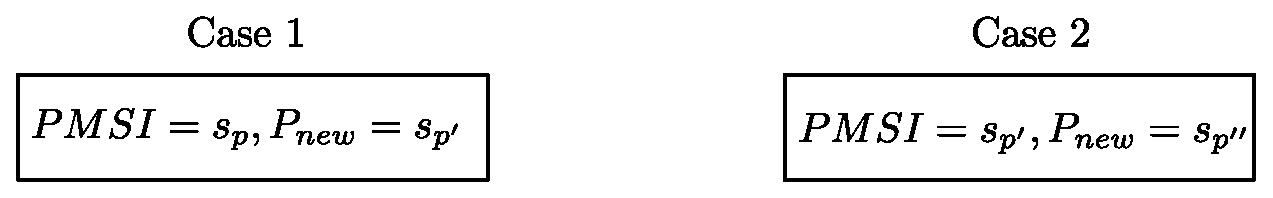
\includegraphics[width=\textwidth]{UE_cases.eps}
  \caption{Values of $PMSI$ and $P_{new}$ in the absence of a malicious or buggy SN}
  \label{fig:ue_cases}	
\end{figure}


Let us assume that a malicious SN has sent a fake location update message for a pseudonym $q$ to an HN. If by chance, the pseudonym $\left(q = s_{p'} \land s_{p''}! = null\right) \vee \left( q = s_{p''}\right)$ for a legitimate subscriber $s$, then the HN forgets $s_p$. To avoid the conditions on $s_{p''}$ being null, the malicious SN might send $AVR_{q}$ so that $s_{p''}$ is set to a non-$null$ value. Consequently, the attack consists of two consecutive messages. The malicious SN first sends $AVR_q$ and wait. After receiving the $AV$ from the HN, the malicious SN sends $LU_{q}$ to the HN. The attack has two phases: 

\subsubsection{Phase 1}  The malicious SN sends $AVR_{q_1}$ and $LU_{q_1}$. If by chance, $\left(q_1 = s_{p'} \right) \vee \left(q_1 = s_{p''}\right)$, then the HN forgets $s_p$. At this stage the state of the subscriber at HN becomes $(s_i,s_p,s_{p'},null,0)$. The situation of the subscriber in the UE becomes $\left(PMSI \notin \left\lbrace s_p,s_{p'} \right\rbrace, P_{new} = s_{p} \right)$

\subsubsection{Phase 2} The malicious SN sends $AVR_{q_2}$ and $LU_{q_2}$. If by chance, $\left(q_2 = s_{p'} \right)$, then the HN forgets $s_p$. At this stage the state of the subscriber at HN remains $(s_i,s_p,s_{p'},null,0)$. The situation of the subscriber in the UE becomes $\left(PMSI \notin \left\lbrace s_p,s_{p'} \right\rbrace, P_{new} \notin \left\lbrace s_p, s_{p'}  \right\rbrace \right)$

\subsection{Probality of Success of the Attack}
A malicious SN has to successfully guess two pseudonyms $q_1,q_2$ to affect a subscriber $s$. However, if the subscriber $s$ is currently connected to the malicious SN, $q_1$ does not need to be guessed. The SN can collect the $P_{new}$ of all the subscribers connected to it by making identity requests to the UEs. Then for each $P_{new}$, the malicious SN performs the Phase 1 of the attack discussed in Section \ref{sec:attack_by_sn}. 

However, the malicious SN has no way to know the new $s_{p'}$ the HN has set for a subscriber $s$ after the Phse 1 of the attack. Consequently the HN has to guess $q_2$ to mount the second phase of the attack. If the malicious SN guesses with replacement, the probability of one guess to be successful in the seond phase is $\frac{r}{10^10}$ where $r$ is the number of subscribers of the HN currently visiting the malicious SN. Figure \ref{fig:expected_success_rate_attack_by_sn_insider} shows the expected number of affected subscribers as the number of guess grows. The expected number of affected subscribers are computed as $\left(1-\left(1-\frac{1}{10^{10}}\right)^m\right))$ where $m$ is the number of pseudonyms guessed. However, if the pseudonyms are guessed without replacement, the number of affected user will be a bit higher. But we believe it will still be very insignificant comparing with the number of pseudonyms have to be guessed. The malicious SN can be detected and be blocked far before it reaches guessing $1$ million pseudonyms 

\begin{figure}[]
  \centering
    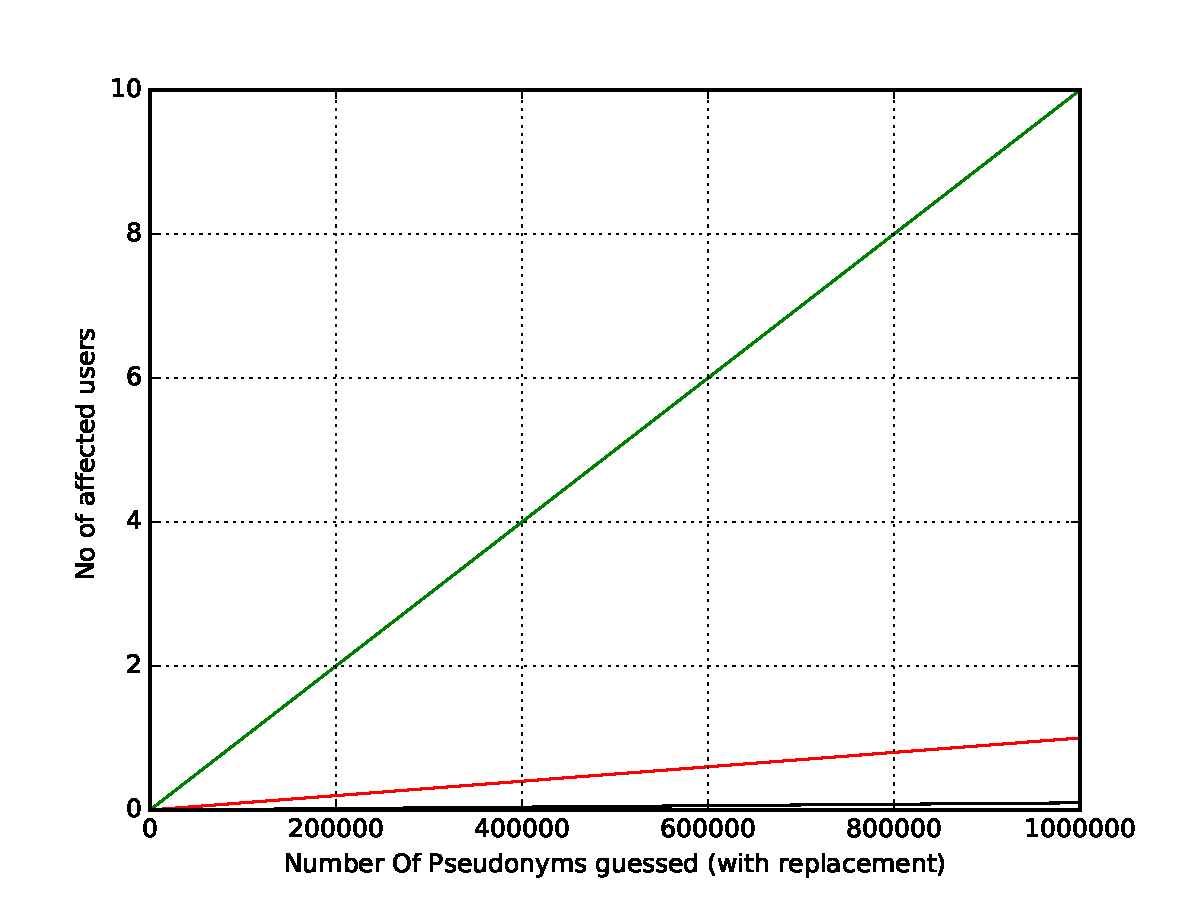
\includegraphics[width=\textwidth]{expected_success_rate_attack_by_sn_insider.pdf}
  \caption{Expected number of affected subscriber in the attack by SN. The attack is targeted to the subscribers who are visiting the SN}
  \label{fig:expected_success_rate_attack_by_sn_insider}	
\end{figure}


However, the malicious SN can target the subscribers of an HN who are not even visiting the malicious SN. In that case the malicious SN has to guess both of the pseudonyms $q_1$ and $q_2$. If the pseudonyms are guessed without replacement then the expected number of affected subscribers would be as following:

\begin{eqnarray}
E\big[ u_a \big] = \begin{cases} \frac{1}{10^{10}}\frac{m^2}{2\cdot 10^{10}} \times r, & \mbox{if } 0 < m \leq 10^{10} \\ 
\frac{1}{10^{10}}(2m - 10^{10} - \frac{m^2}{2\cdot 10^{10}}) \times r, & \mbox{if } 10^{10} < m \leq 2\cdot 10^{10} \end{cases}
\label{eqn:without_replacement}
\end{eqnarray} 

Figure shows how it grows as $m$ grows with varied $r$

\begin{figure}[]
  \centering
    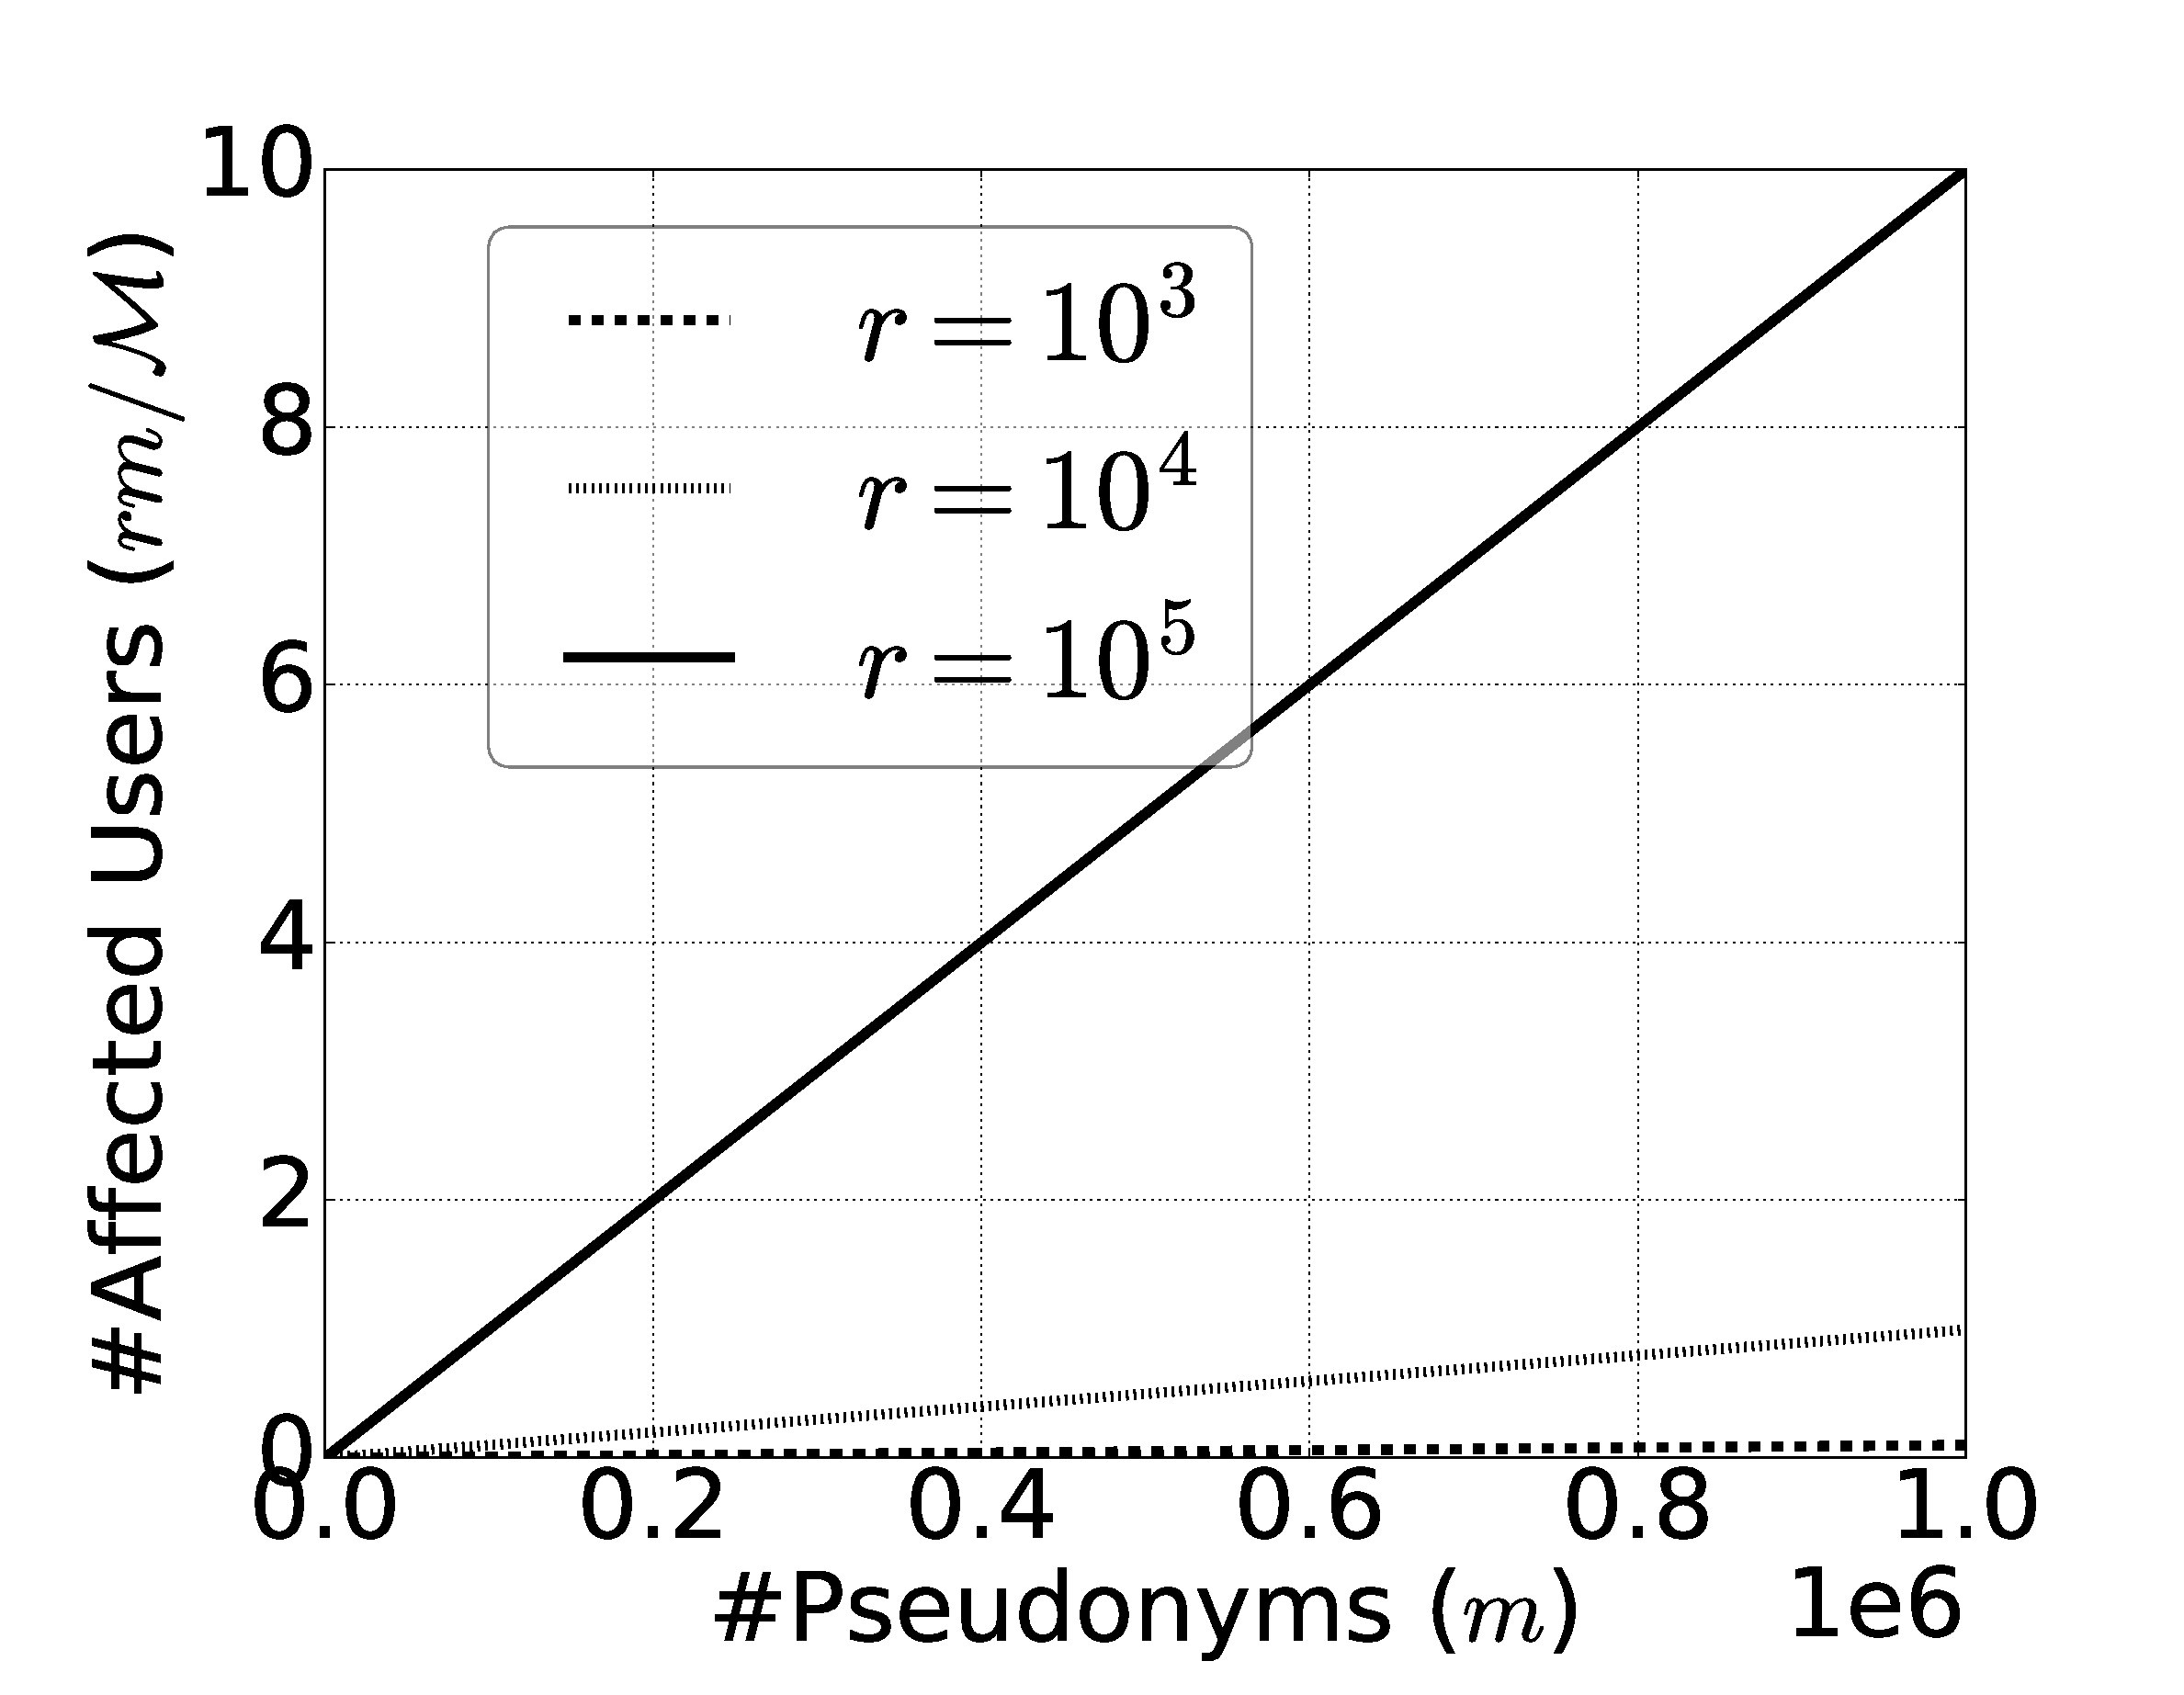
\includegraphics[width=\textwidth]{sn_attack_all.pdf}
  \caption{Expected number of affected subscriber in the attack by SN. The attack is targeted to all subscribers of the HN}
  \label{fig:expected_success_rate_attack_all_by_sn}	
\end{figure}


\section{Usability of pseudonyms}



\section{Conclusion}
\label{sec:conclusion}


\subsubsection{Acknowledgement.}
\label{sec:acknowledgement}


\bibliographystyle{splncs}
\bibliography{ref}{}

\begin{thebibliography}{5}



\end{thebibliography}

\end{document}
